%! TEX root = 'main.tex'
\section{Reverse Engineering and Design}
\label{sec:implant-design}


The major challenge in making a PLC-specific hardware backdoor is that PLC does not use open standards like PC.  During the development, a significant amount of time is spent on the reverse engineering of the PLC. After a basic understanding of its modules and chips, we can choose how to control it, whether through JTAG or intercepting other low-speed buses.


\subsection{Reverse Engineering}
The PLC we use is Allen-Bradley 1769-L18ER-BB1B/B CompactLogix 5370.
The reverse engineering work includes both the hardware and software parts. First, we speculate on the function of each board of the PLC. Then we identify the on-board IC chips and use a multimeter to conduct the connectivity test for wire tracing. The purpose of this is to find the interconnections between chips and between boards. Fortunately, the real-time module is a two-side PCB, and the wire connectors that pass through the board are well exposed, as seen in~\autoref{fig:ssi0}. Furthermore, we dump the firmware from the microcontroller and flash chip for reverse-engineering analysis.


\textbf{\textit{Backplanes.}} The Allen Bradley PLC contains several PCB module boards, known as backplanes. ~\autoref{fig:modules} shows each module. In this paper, we name the board with the Ethernet socket and USB port as the communication module (\textbf{B}).  The one controls that has a microcontroller and controls the 16 digital DC input pins and 16 digital DC output pins as the real-time module {\textbf{C}}, which is our main target. Module \textbf{D} is merely a connector for the digital IO. The rest are the power supply module(\textbf{A}) and LED module(\textbf{E}).


The communication module (\textbf{B}) itself is an embedded system, including a CPU, DRAM, and other peripherals such as Ethernet, SD card, and USB.  It communicates with the host (HMI) to receive firmware and ladder logic updates, and it also hosts a web server to display status. However, this module does not directly interact with IO. By analyzing the PLC firmware update files, we find that this board runs VxWorks operating system. Nevertheless, this board's primary chip is an FPGA~\cite{kuon2008fpga} chip that runs a soft-core ARM processor, and it is in BGA packaging. It is not easy to trace and identify which GPIO pins of the FPGA are used as the JTAG interface. We consider it as one of our further works. Therefore, our focus is the real-time module (\textbf{C}) that runs ladder logic and directly controls IO. Fortunately, this module uses a commercial microcontroller, namely, Texas Instruments Stellaris LM3S2793 SoC.

The digital IO sockets on the connector module (\textbf{D}) connects to the real-time module (\textbf{B}). The IO goes through the power switches and optically coupled isolator chips and eventually connects to the microcontroller, as shown in~\autoref{fig:board}. There are 32 LEDs corresponds to each IO socket, and the real-time module also controls the LED module through the I2C protocol. The power module (\textbf{A}) provides stable 3 volts for other boards. Our backdoor can either get power directly from it or the JTAG pad.

\begin{figure}[th]
	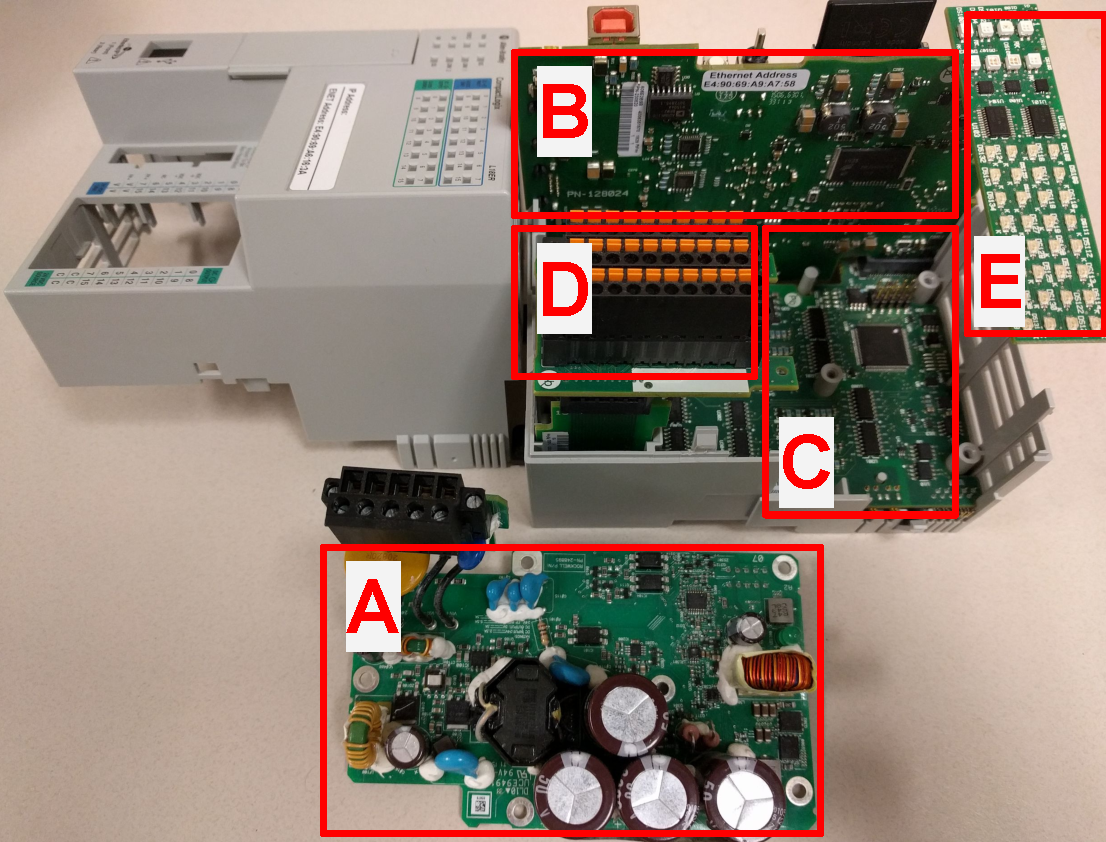
\includegraphics[width=0.47\textwidth]{figures/modules}
	\centering
	\caption{Allen-Bradley 1769-L18ER-BB1B/B CompactLogix 5370 PLC. A: Power supply module  B: Communication module  C: Real-time module  D: (16) DC Digital Outputs \& (16) DC Digital Inputs Connector  E: LED  module}
	\label{fig:modules}
\end{figure}




\textbf{\textit{Microcontroller.}} The TI Stellaris LM3S2793 SoC has an ARM Cortex-M3 processor core that operates at 80 MHz. It contains 64 KB SRAM and 128 KB flash. The internal ROM is preprogrammed with Stellaris Peripheral Driver Library (DriverLib) to drive the on-chip peripheral devices. ~\autoref{tab:memorymap} shows the memory map. 


\begin{center}
	\begin{table}
		\small
		\begin{tabular}{p{1.6cm}  p{1.6cm}  p{4cm}} 
			\hline
			%Start & End & Description \\ [0.5ex] 
			Start & End & Description \\ 
			\hline
			\multicolumn{3}{l}{\textbf{Memory} (0x00000000 - 0x22200000)}  \\
			\hline
			0x00000000 & 0x0001FFFF & On-chip Flash \\ 
			\hline
			0x00020000 & 0x00FFFFFF & Reserved \\
			\hline
			0x01000000 & 0x01004FFF & On-chip ROM  \\
			\hline
			0x01005000 & 0x01005EFF & AES+CRC lib in on-chip ROM   \\
			\hline
			... & & \\
			\hline
			%0x01005F00 & 0x1FFFFFFF & Reserved \\ 
			%\hline
			0x20000000 & 0x2000FFFF & Bit-banded on-chip SRAM \\
			\hline
			... & & \\
			\hline
			%0x20010000 & 0x21FFFFFF & Reserved \\
			%\hline
			%0x22000000 & 0x221FFFFF & Bit-band alias of bit-banded on-chip SRAM starting at 0x20000000 \\
			%\hline
			%0x22200000 & 0x3FFFFFFF & Reserved \\
			\multicolumn{3}{l}{\textbf{FiRM Peripherals} (0x40000000 - 0x4001FFFF)}  \\
			\hline
			... & & \\
			\hline
			0x40008000 & 0x40008FFF & SSI0 \\
			\hline
			... & & \\
			\hline
			\multicolumn{3}{l}{\textbf{Peripherals} (0x40020000 - 0xDFFFFFFF)}  \\
			\hline
			0x40020000 & 0x400207FF & I2C Master 0 \\
			\hline
			... & & \\
			\hline
			0x4005C000 & 0x4005CFFF & GPIO Port E (AHB aperture) \\
			\hline
			0x4005D000 & 0x4005DFFF & GPIO Port F (AHB aperture) \\
			\hline
			0x4005E000 & 0x4005EFFF & GPIO Port G (AHB aperture) \\
			\hline
			0x4005F000 & 0x4005FFFF & GPIO Port H (AHB aperture) \\
			\hline
			... & & \\
			\hline
			\multicolumn{3}{l}{\textbf{Private Peripheral Bus} (0xE0000000 - 0xFFFFFFFF)}  \\
			\hline
			... & & \\
			\hline
			0xE000E000 & 0xE000EFFF & Nested Vectored Interrupt Controller (NVIC) \\
			\hline
			... & & \\
			\hline
		\end{tabular}
		\caption{LM3S2793 Memory Map. Only list the address space of the memory and devices related to this paper. FiRM-compliant (compliant to the ARM Foundation IP for Real-Time Microcontrollers specification).}
		\label{tab:memorymap}
	\end{table}
\end{center}


\textbf{\textit{Reset Vector.}} The vector table is at a fixed address 0x00000000 after the system reset. The core starts to execute from memory 0x00000004, which is the reset vector. ~\autoref{tab:memorymap} shows that the reset vector resides in the flash memory instead of the ROM. It is because the ROM boot loader is only executed in two scenarios. The first case is when the flash memory is empty. The other one is when an application initiates a firmware update and calls the ROM boot loader to execute. For instance, if data at 0x00000004 is 0xFFFFFFFF, which indicates an empty flash, then the ROM is mapped to 0x00000000 to substitute the flash and execute instead. 

The data at 0x00000000 and 0x00000004 will be loaded into the stack pointer (SP) and the program counter (PC), respectively. In our case, the SP is 0x20000B48, and the PC is 0x000000E3. Notice that 0xE3 is an odd number. As we know, RISC processors such as ARM uses fixed-length instruction. On ARM processors, setting the PC's least significant bit indicates that the following code will be executed as the two-byte Thumb instructions. Therefore, we dump the flash memory and disassemble it at address 0x000000E2 instead.



\textbf{\textit{Flash Boot Loader.}} Right after the flash boot loader starts, it copies itself to SRAM, starting at 0x20000000. Although both SRAM and flash memory can be accessed in a single cycle, flash memory can do that as long as the code is linear and branches incur a one-cycle stall. The bootloader copies 0x00000000 - 0x00000A88 to 0x20000000 - 0x20000A88, and clear the data section (0x20000A88 - 0x20000F54). As mentioned earlier, on system reset, the vector table is at the fixed address 0x00000000. However, it can be relocated by writing the vector table offset register (VTOR:0xE000ED08). Changing the vector table indicates a complete change of the system's behavior because all the interrupt handlers are new, and they interpret how the system behaves regarding peripheral device's requests. The bootloader sets the vector table to 0x20000000 and jumps back to SRAM to continue execution.


\textbf{\textit{Stellaris Peripheral Driver Library.}} The Drivelib~\cite{lm3s2793rom} is a set of APIs utilized to control the on-chip peripheral devices. It is provided in ROM code and placed in a fixed location on Cortex-M3 SoCs. It helps identify what functions the firmware calls. Through the fixed location of APIs and the Drivelib datasheet, the function matches with names. It is a two-level table structure. The main table is at 0x1000010, and it contains the address of the second-level table for each type of peripherals, as shown in~\autoref{tab:romtable}. For example, ~\autoref{tab:gpiotable} shows the \texttt{ROM\_GPIOTABLE}, which contains all the GPIO related APIs.

\begin{center}
	\begin{table}
		\small
		\begin{tabular}{|p{7.2cm}|} 
			\hline
			\texttt{ROM\_APITABLE (0x1000010)} \\ %[0.5ex] 
			\hline
			[0] = \texttt{ROM\_VERSION} \\
			\hline
			[1] = pointer to \texttt{ROM\_UARTTABLE} \\
			\hline
			[2] = pointer to \texttt{ROM\_SSITABLE} \\
			\hline
			[3] = pointer to \texttt{ROM\_I2CTABLE} \\
			\hline
			[4] = pointer to \texttt{ROM\_GPIOTABLE} \\
			\hline
			[5] = pointer to \texttt{ROM\_ADCTABLE} \\
			\hline
			... \\ 
			\hline
		\end{tabular}
		\caption{LM3S2793 ROM API table is at a fixed address 0x1000010, and each table entry is 4 bytes address that points to a second-level table, which corresponds to a class of peripheral devices.}
		\label{tab:romtable}
	\end{table}
\end{center}

\begin{center}
	\begin{table}
		\small
		\begin{tabular}{|p{7.2cm}|} 
			\hline
			\texttt{ROM\_GPIOTABLE} \\ [0.5ex] 
			\hline
			[0] = function \texttt{ROM\_GPIOPinWrite} \\
			\hline
			[1] = function \texttt{ROM\_GPIODirModeSet} \\
			\hline
			[2] = function \texttt{ROM\_GPIODirModeGet} \\
			\hline
			[3] = function \texttt{ROM\_GPIOIntTypeSet} \\
			\hline
			[4] = function \texttt{ROM\_GPIOIntTypeGet} \\
			\hline
%			[5] = function ROM\_GPIOPadConfigSet \\
%			\hline
			... \\ 
			\hline
		\end{tabular}
		\caption{GPIO API Table. Each table entry is the entry address of an API, and the function parameters are passed through registers. There is no privilege or mode change when calling into the APIs.}
		\label{tab:gpiotable}
	\end{table}
\end{center}



\autoref{fig:romapiexample} shows a typical code snippet that calls a ROM API. The second-level table is at 0x1000010 + 0x10 (\texttt{ROM\_APITABLE[4]}), which is the the GPIO table. And the API it calls is \texttt{ROM\_GPIOPinRead()} (\texttt{ROM\_GPIOTABLE[11]}). Because all the ROM API call sites have the same pattern, it makes firmware's reverse engineering work much easier.  Calling the API is merely locating the function address from the two-level tables and jumps to it, and the parameters are passed in through registers. There is no privilege change when calling into the APIs, and the firmware code all runs in the system mode.


\begin{figure}[th]
	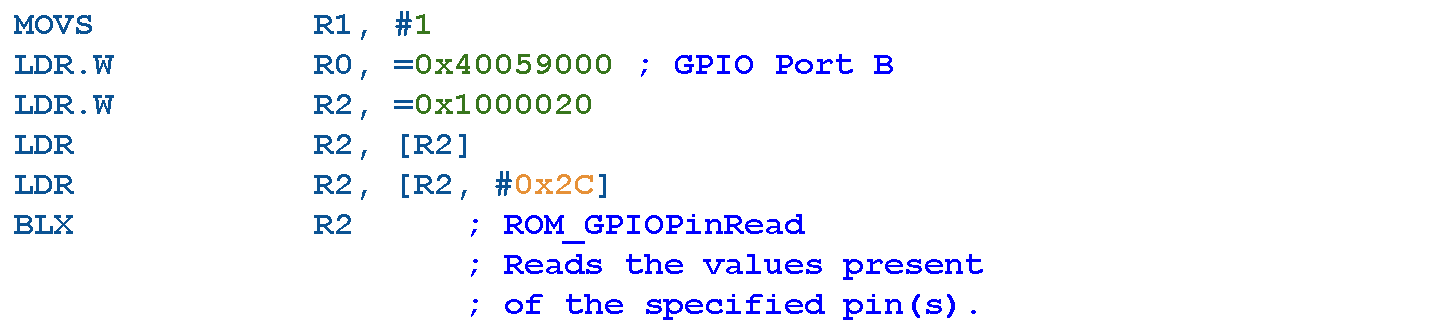
\includegraphics[width=0.47\textwidth]{figures/romapiexample2}
	\centering
	\caption{A code snippet that calls \texttt{ROM\_GPIOPinRead()}. The parameters are passed through registers. In this case, the  \texttt{ROM\_GPIOPinRead()} has two parameters. R0 contains the GPIO port address, and R1 indicates the pins to operate.}
	\label{fig:romapiexample}
\end{figure}




%\textbf{\textit{Debug.}} In addition to reverse-engineering,  we also need to debug the firmware. We use the SEGGER J-Link debugger. Since the target is ARM and the debugger sets up a GDB server, we also need GNU Embedded Toolchain for ARM~\cite{gnutoolchainarm}, an ARM version of the gdb client.
%
%
%As mentioned earlier, the stack pointer and program counter are located at address 0x00000000 and 0x00000004. As shown in~\autoref{fig:gdbinit}, we use a GDB initialization script that contains GDB commands to set up the target. This script makes the PLC initialized and runs ladder logic, but the PLC cannot be interrupted during runtime with the debugger. If so, the indicator on the LED panel will prompt an IO error. The reason is still under investigation, and it could be that the watchdog timer is not handled well.
%
%\begin{figure}[th]
%	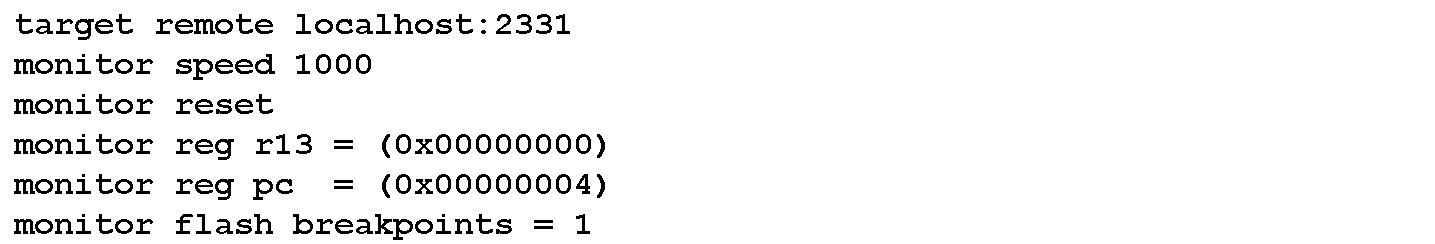
\includegraphics[width=0.47\textwidth]{figures/gdbinit}
%	\centering
%	\caption{The minimal gdbinit script that sets the SP and PC registers makes the PLC be up and running. Other on-chip peripheral controllers may not be correctly initialized.}
%	\label{fig:gdbinit}
%\end{figure}
%


%\subsubsection{more reverse engineering topics ....}

%Through reverse engineering, it shows that the Vector Table Offset Register is first at address 0x0, then switch to address 0x20000000, after receiving the ladder logic code, finally set to address 0x40000. 



\textbf{\texttt{GPIO.}} The PLC interacts with the physical world through digital inputs and outputs. The IO goes through the power switches and optically coupled isolator chips and eventually connects to the microcontroller's GPIO.


In the microcontroller LM3S2793, the GPIO module comprises nine physical GPIO blocks, and each corresponds to an individual GPIO port. Depending on the microcontroller's configuration, it supports up to 67 programmable input/output pins or several pins grouped to provide peripheral functions such as I2C. The GPIO ports can be accessed either through AHB or APB bus, which matters when we access the GPIOs through JTAG. We choose the AHB-AP.

Each GPIO port has several associated control registers, such as GPIO Digital Enable (GPIODEN), GPIO Alternate Function Select (GPIOAFSEL), GPIO Port Control (GPIOPCTL), and GPIO Data Control registers. All GPIO pins are configured as individual input/output pins and tri-stated by default. The GPIO Direction (GPIODIR) register configures each GPIO pin as an input or output, and we do not change it. To change the inputs and outputs, we primarily operate on the GPIO Data (GPIODATA) register that modifies individual bits in GPIO ports. 

The way to control the GPIO data is not straightforward.  Different microcontrollers adopt different operating methods. For example, the GPIO port may take Output Data Register (ODR), Bit Reset Register (BRR), Bit Set/Reset Register (BSRR)~\cite{cottle2001programmable}. In our case, the LM3S2793 microcontroller uses a more complicated model to conduct bit-wise operations. The GPIO Data register is memory-mapped. When read/write, bits[9:2] of the address are treated as a bitmask, as well as the bits[1:0] are always zero because the memory access should be at 4-byte alignment on ARM. Therefore, for each GPIO port, the memory-mapped range should be 1KB long, that is, from GPIODATA to GPIODATA + 0x3FC. A write can only change the data bit when the corresponded bitmask is set. Otherwise, the data bit is unchangeable.

For example, GPIO Port A (AHB) is mapped at 0x40058000, and it controls 8 GPIO pins. We want to set bit2 to 0 and bit5 to 1. As shown in~\autoref{fig:gpiowrite}, the bitmask is 0x90, and the data is 0xF0.  Hence, the operation should be writing 0xF0 to address 0x40058090.


\begin{figure}[th]
	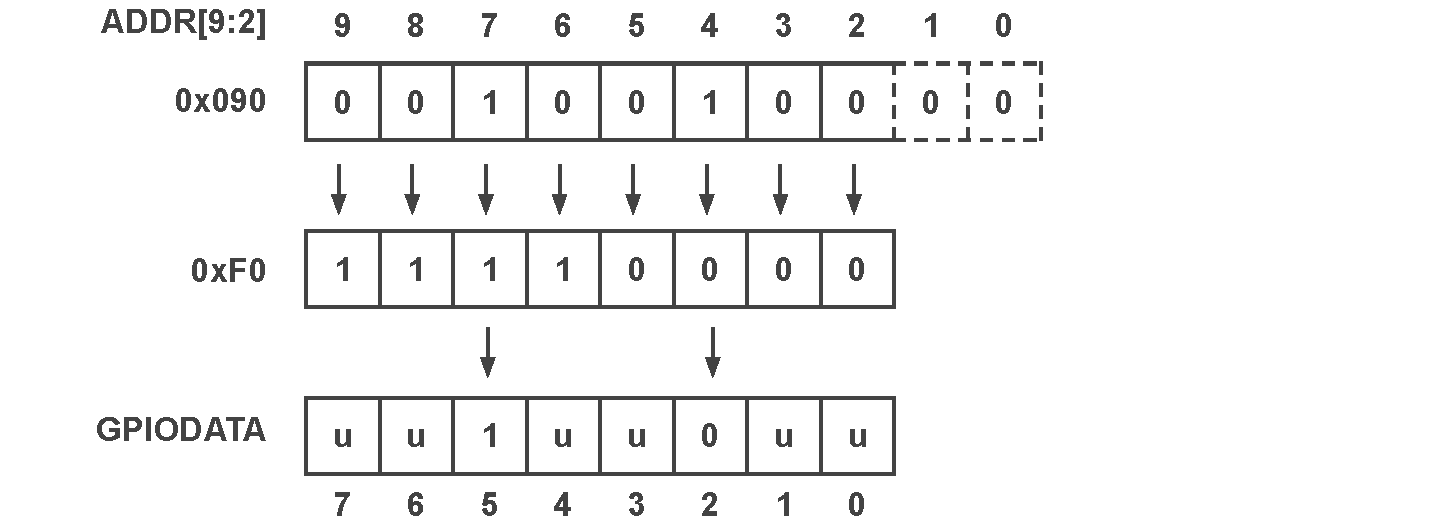
\includegraphics[width=0.47\textwidth]{figures/gpiowrite2}
	\centering
	\caption{Writing a byte of 0xF0 to address GPIODATA + 0x90.  The bitmask only allows bit2 and bit5 to be modified. Therefore, only two bits are valid for the write operation.  \textbf{u} indicates the new bit is ignored.}
	\label{fig:gpiowrite}
\end{figure}



The same applies to reading. Only the corresponding bit in the bitmask will be read. Otherwise, it reads zero. For example, to read the four high bits from GPIO Port A, the address with bitmask should be 0x40058000 + 0x3C0, and it reads 0xA0, as shown in~\autoref{fig:gpioread}.

\begin{figure}[th]
	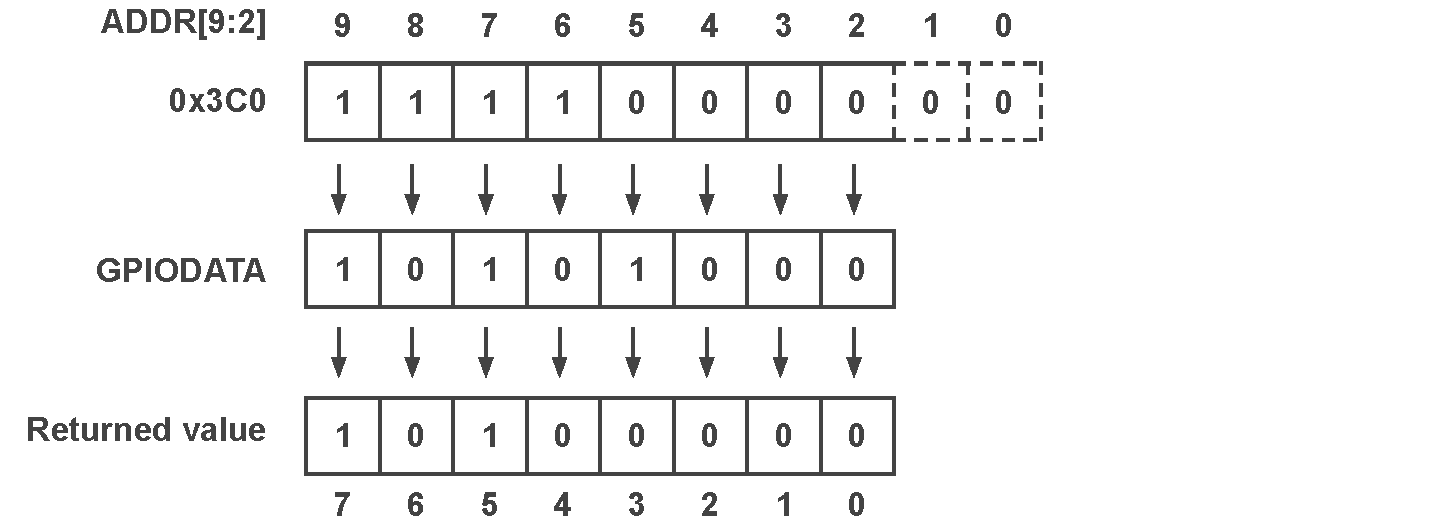
\includegraphics[width=0.47\textwidth]{figures/gpioread2}
	\centering
	\caption{The address GPIODATA+0x3C0 reads the high four bits of the GPIO port. The rest reads zero regardless of the actual value.}
	\label{fig:gpioread}
\end{figure}



\textbf{\texttt{Control Output.}} After knowing how to control GPIO, we can directly control the output of the PLC. There are 16 inputs and 16 outputs on the IO connector. Through reverse engineering, we know the GPIO port corresponding to the IO.  That are, GPIO port E (0x4005C000) GPIO port F (0x4005D000) for inputs, and GPIO port G (0x4005E000), GPIO port H (0x4005F000) for outputs. Intuitively, each GPIO bit corresponds to a pin on the connector. One indicates the high voltage, which is the field power voltage; zero dictates the low voltage (8 volts).

To conduct a stealthy attack, we want to change the output secretly. For example, we want to keep the LEDs in their original state and the host (HMI) not to find any abnormalities. To achieve this goal, we need to leverage the firmware itself. The PLC periodically scans the inputs, runs ladder logic, and updates outputs.  It is trivial to find the ladder logic binary by following the timer handler routine. There are a few local variables that control how the ladder logic behaves. For example, one local variable determines if any logic state has changed. If so, the corresponded GPIO pin will be updated according to the ladder logic. We modify this local variable so that everything looks up to date. In the meantime,  we can change the outputs without triggering any alarms.



\textbf{\textit{AT45DB021E SPI Flash Memory.}}  It is quite noticeable that right next to the LM3S2793 microcontroller,  there is an 8-pin flash chip, which is an Adesto 45DB021E 2-Mbit SPI flash memory. It connects with the PLC's SSI0 (Synchronous Serial Interface), as shown in ~\autoref{fig:ssi0}.

\begin{figure}[th]
	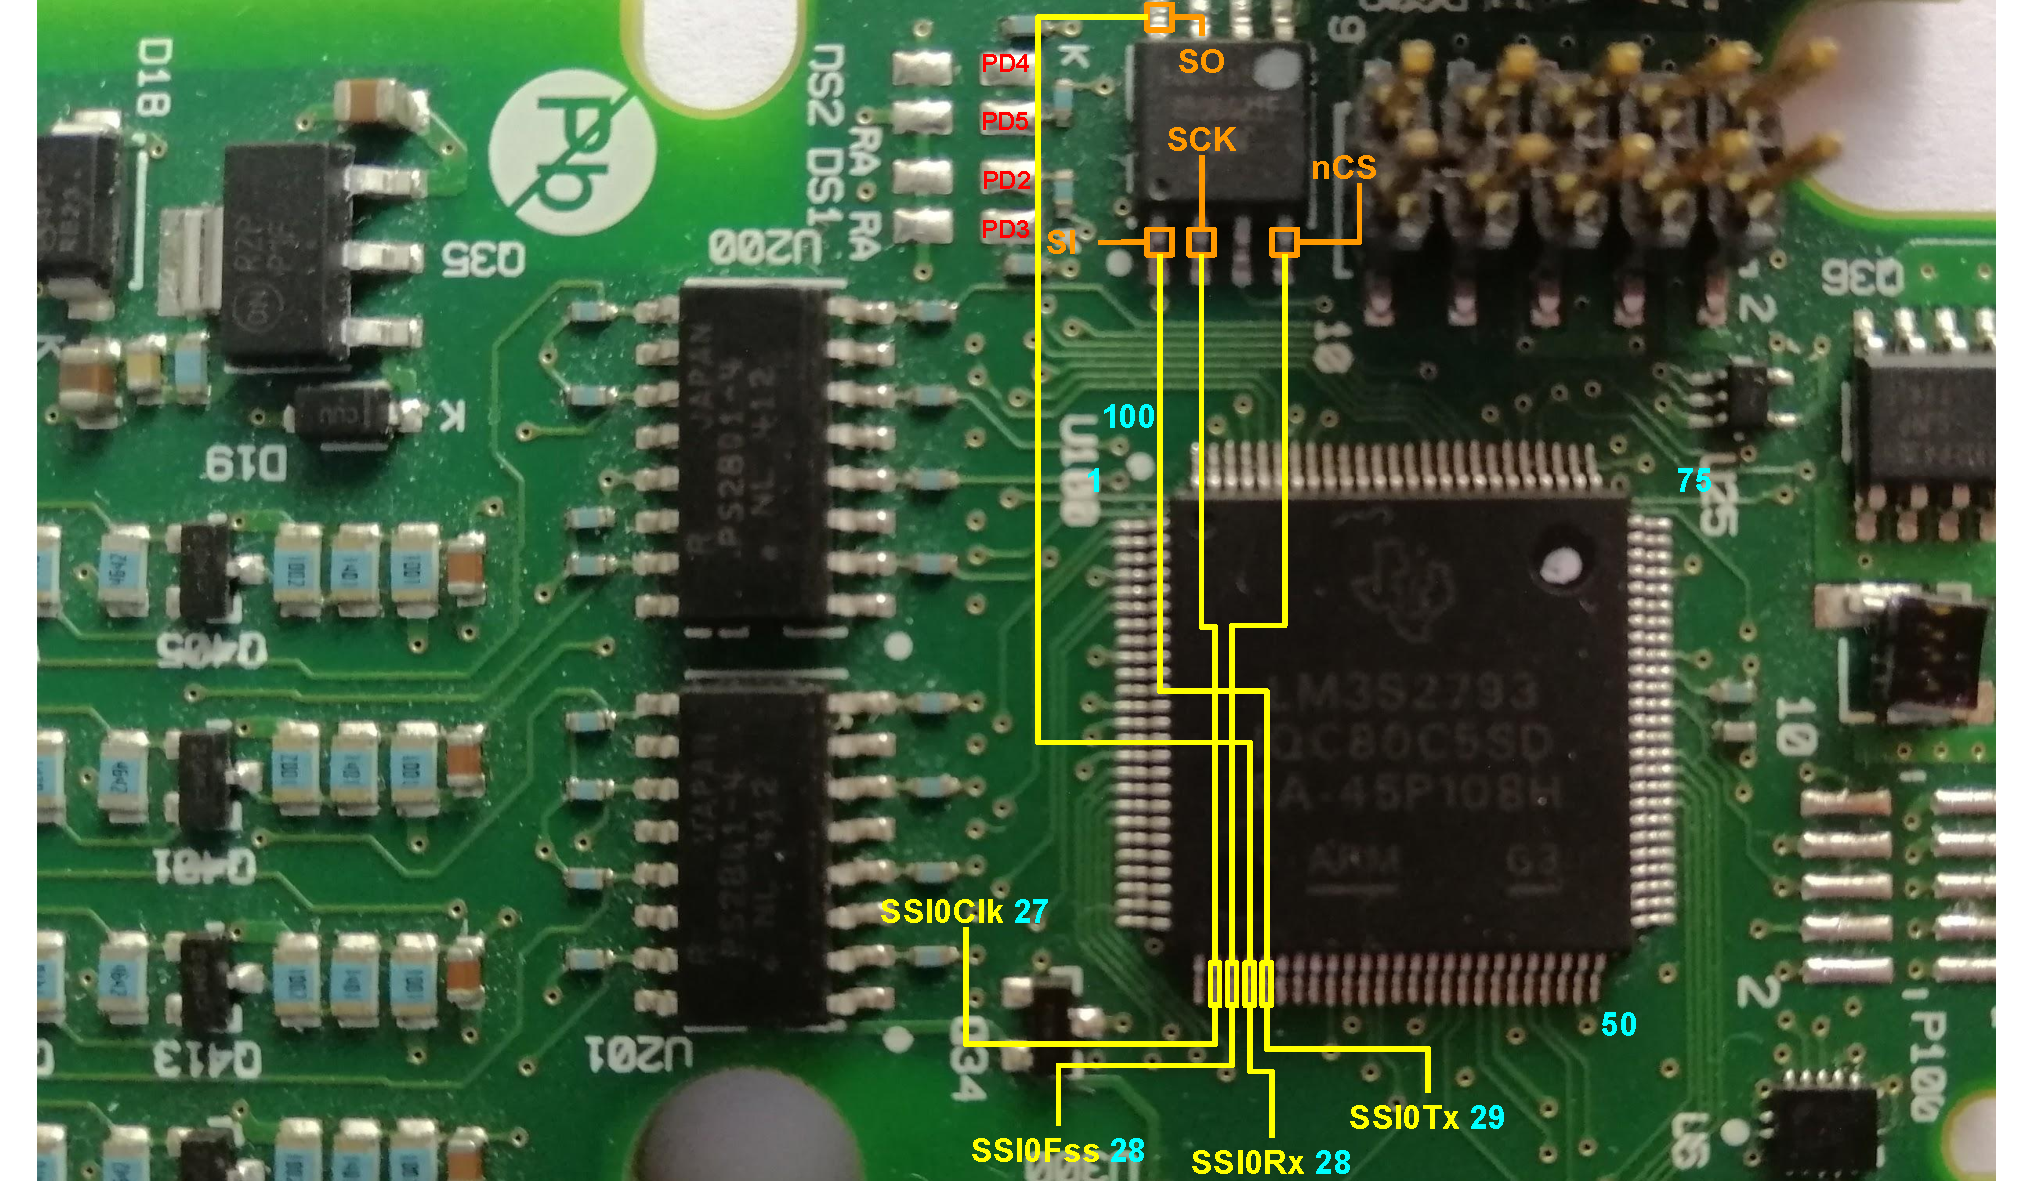
\includegraphics[width=0.47\textwidth]{figures/ssi0}
	\centering
	\caption{Through wiring tracing, we find that the AT45DB21E SPI Flash Memory connects to LM3S2793's SSI0 interface. The eight solder joints on the left may be used to install four LEDs. They are controlled by GPIO port D,  but they are not installed.}
	\label{fig:ssi0}
\end{figure}


During the boot process, the pins in GPIO port A are assigned for the SSI0 master device. The firmware first reads one byte from the flash chip (offset 0x2000), which looks like a status byte. If it equals 0x55 or 0xAA, the PLC will be reset. If not, the firmware checks the integrity of the address 0x4000 to 0x1FFFC, the compiled ladder logic. The algorithm is a simple checksum. Accumulate each byte in this address range, and the result should be equal to the byte in address 0x1FFFF.

So this status byte at 0x2000 indicates the status of the PLC last time it was running. The value 0x55 indicates that the system has encountered a severe failure. If so, the firmware operates on GPIO port D, leading to the eight solder joins next to the SPI flash. We think they may be four LEDs to show the status. Furthermore, if the value is 0xAA, it means that the ladder logic binary has been broken, and the firmware will copy the code from 0x6100 in the SPI flash. We think this is a backup code and also a place where malicious code can be stored.

To read the AT45DB21E flash chip's content, we port its driver to the Teensy 3.2 board. The source code is available at the github~\footnote{https://github.com/whensungoesdown/at45db021\_teensy32}.



\textbf{\textit{Front Panel LED.}} There are four rows of LEDs on the front panel of the PLC. Each LED represents the state of an input or output. Usually, this is a very intuitive reflection of the current status of the PLC.

There are four rows of LED lights on the PLC's front panel. Each LED shows individual input and output pins' status, which is an intuitive way for the administrator to check whether the device works properly. The microcontroller controls these LEDs through the I2C protocol~\cite{semiconductors2000i2c}.

There are two 24-pin PD9535 chips (Remote 16-bit I2C/SMBus, Low-Power I/O Expander~\cite{pd9535}) on module \textbf{E}. It provides general-purpose I/O expansion for microcontrollers via the I2C bus. The two pins in GPIO port B(PB2 and PB3) on the microcontroller are used as the SCL and SDA signal lines for the I2C master device. These two signal lines also pass through the connector between module \textbf{B} and \textbf{C}, as shown in~\autoref{fig:p607}.

Each I2C slave device on the same bus has a unique 7-bit address. In our example, the addresses of the two PD9593 chips are 0x20 and 0x21. ~\autoref{tab:i2ccommand} shows that the chip has eight internal registers. As mentioned in~\autoref{sec:implant-background}, after the master device successfully sends the address byte, it will send another byte to select the internal register. Among these internal registers, the configuration register is responsible for controlling the directions of the IO pins. Zero means the corresponding pin is output. Because the PLC uses PD9593 to control the LED, all the pins are outputs. The input port registers reflect the pins' incoming logic levels, regardless of whether the pin is defined as an input or an output by the configuration register. Nevertheless, we do not need to read the input registers.



\begin{center}
	\begin{table}
		%\begin{tabular}{|c|@{}c@{}|c|c|} 
		\begin{tabular}{|@{}>{\centering\arraybackslash}m{0.9cm}@{}|
				@{}>{\centering\arraybackslash}m{3.65cm}@{}|
				@{}>{\centering\arraybackslash}m{2.52cm}@{}|
				@{}>{\centering\arraybackslash}m{1.62cm}@{}| }
			\hline
			\makecell{CMD \\Byte} & Register & Protocol & \makecell{Power-up \\Default}\\
			\hline
			0x00 & Input Port 0 & Read byte & xxxx xxxx\\ 
			\hline
			0x01 & Input Port 1 & Read byte & xxxx xxxx\\
			\hline
			0x02 & Output Port 0 & Read/Write byte & 1111 1111\\
			\hline
			0x03 & Output Port 1 & Read/Write byte & 1111 1111\\
			\hline
			0x04 & Polarity Inversion Port 0 & Read/Write byte & 0000 0000\\
			\hline
			0x05 & Polarity Inversion Port 1 & Read/Write byte & 0000 0000\\
			\hline
			0x06 & Configuration Port 0 & Read/Write byte & 1111 1111\\
			\hline
			0x07 & Configuration Port 1 & Read/Write byte & 1111 1111\\
			\hline
		\end{tabular}
		\caption{The internal registers of the PD9593 are selected by the master device sending the command byte. To control the LED, we need to operate the control register and the output register and keep the two polarity inversion registers' default value.}
		\label{tab:i2ccommand}
	\end{table}
\end{center}


\autoref{fig:ledi2cinit} shows the pseudo-code to initialize the I2C IO expander using the ROM API. It first enables the I2C master device and sets the clock frequency to be the same as the microcontroller. After that, call \texttt{ROM\_I2CMasterSlaveAddrSet()} to select the target device's address, whether to send or receive data. Then call \texttt{ROM\_I2CMasterDataPut()} to set the data to be sent next. Only after calling \texttt{ROM\_I2CMasterControl()}, the data will be sent out. In our example, two bytes with content zero are sent to Configuration Port0 and Port1. This operation sets a total of 16 pins as output mode.



\begin{figure}[th]
	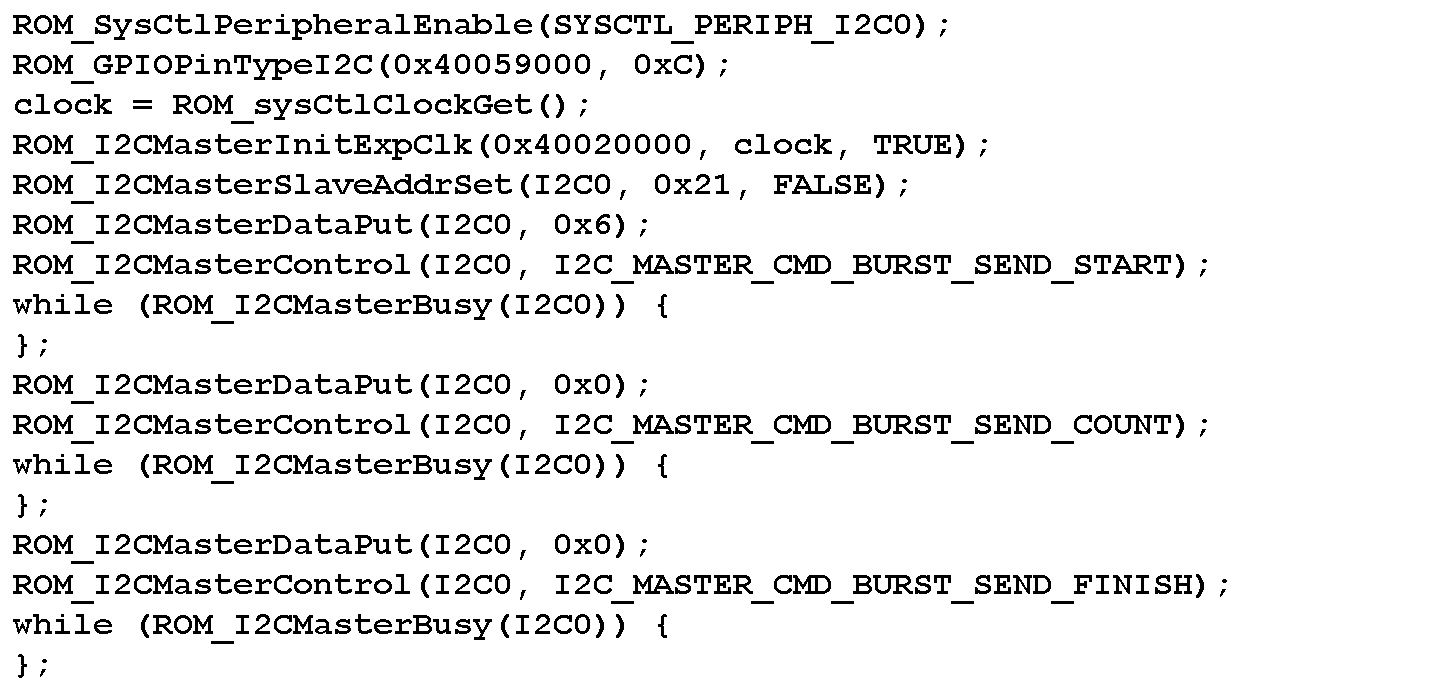
\includegraphics[width=0.47\textwidth]{figures/ledi2cinit}
	\centering
	\caption{The pseudo-code to initialize the I2C IO expander is reversed-engineered from the firmware. To make it more intuitive, we use some macro definitions as parameters. These macros' actual value is not difficult to find in the header files released by the vendor. The code is provided to help understand how to control the LED lights on the PLC through the I2C bus.}
	\label{fig:ledi2cinit}
\end{figure}



After initialization, \autoref{fig:ledi2csend} shows how to control the LEDs. For example, we send two bytes with content 0xFF to the Output Port0 and Port1, lighting up 16 LED lights controlled by this device.


\begin{figure}[th]
	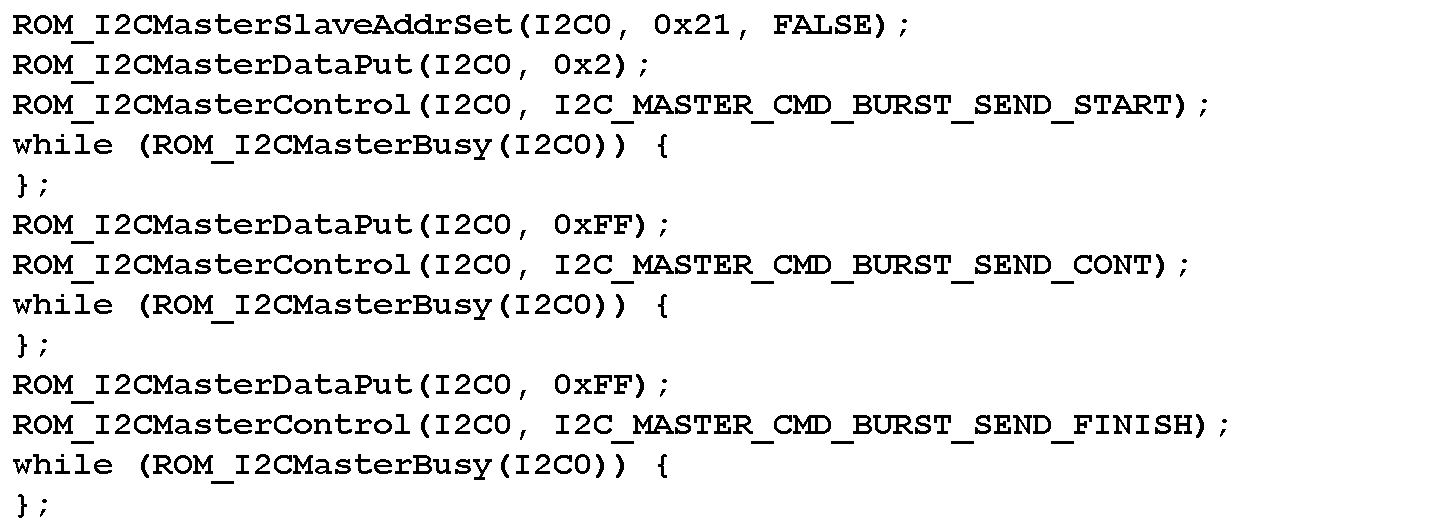
\includegraphics[width=0.47\textwidth]{figures/ledi2csend}
	\centering
	\caption{Each pin in the Output register controls an LED light separately, so two 0xFF bytes can control 16 LEDs. If we only want to control a few of the LED lights in one register, we can call \texttt{ROM\_I2CMasterControl() }with parameter \texttt{I2C\_MASTER\_CMD\_SINGLE\_SEND}.}
	\label{fig:ledi2csend}
\end{figure}






\textbf{\textit{Onboard Connectors.}} There are several connectors on the real-time module \textbf{C}, as shown in ~\autoref{fig:board}. P607 connects to the communication module \textbf{B} and P609 connects to the power module \textbf{A}. Usually, we think that the module \textbf{A} is just a power module responsible for providing three volts to others. However, this is a good place for purposefully damage the PLC by a short circuit, where the power flow is large.

By conducting the connectivity tests with a multimeter, we perceive some pins' function in P607 as shown in~\autoref{fig:p607}. As mentioned earlier, the I2C bus passes through this connector. Besides, the CAN bus also passes through this connector. In this way, both the communication module and the real-time module are connected to the CAN bus connector in the bottom right corner in ~\autoref{fig:board}. These two modules can not only control the external CAN bus device, but they can also communicate via the CAN bus themself. However, the communication module has a higher priority. Setting pin29 on the P607 connector can block the transmission of the signal on pin21, the CAN bus's RxD signal line. On the microcontroller side, the master device CAN0 uses the PA6 and PA7 pins. 


\begin{figure}[th]
	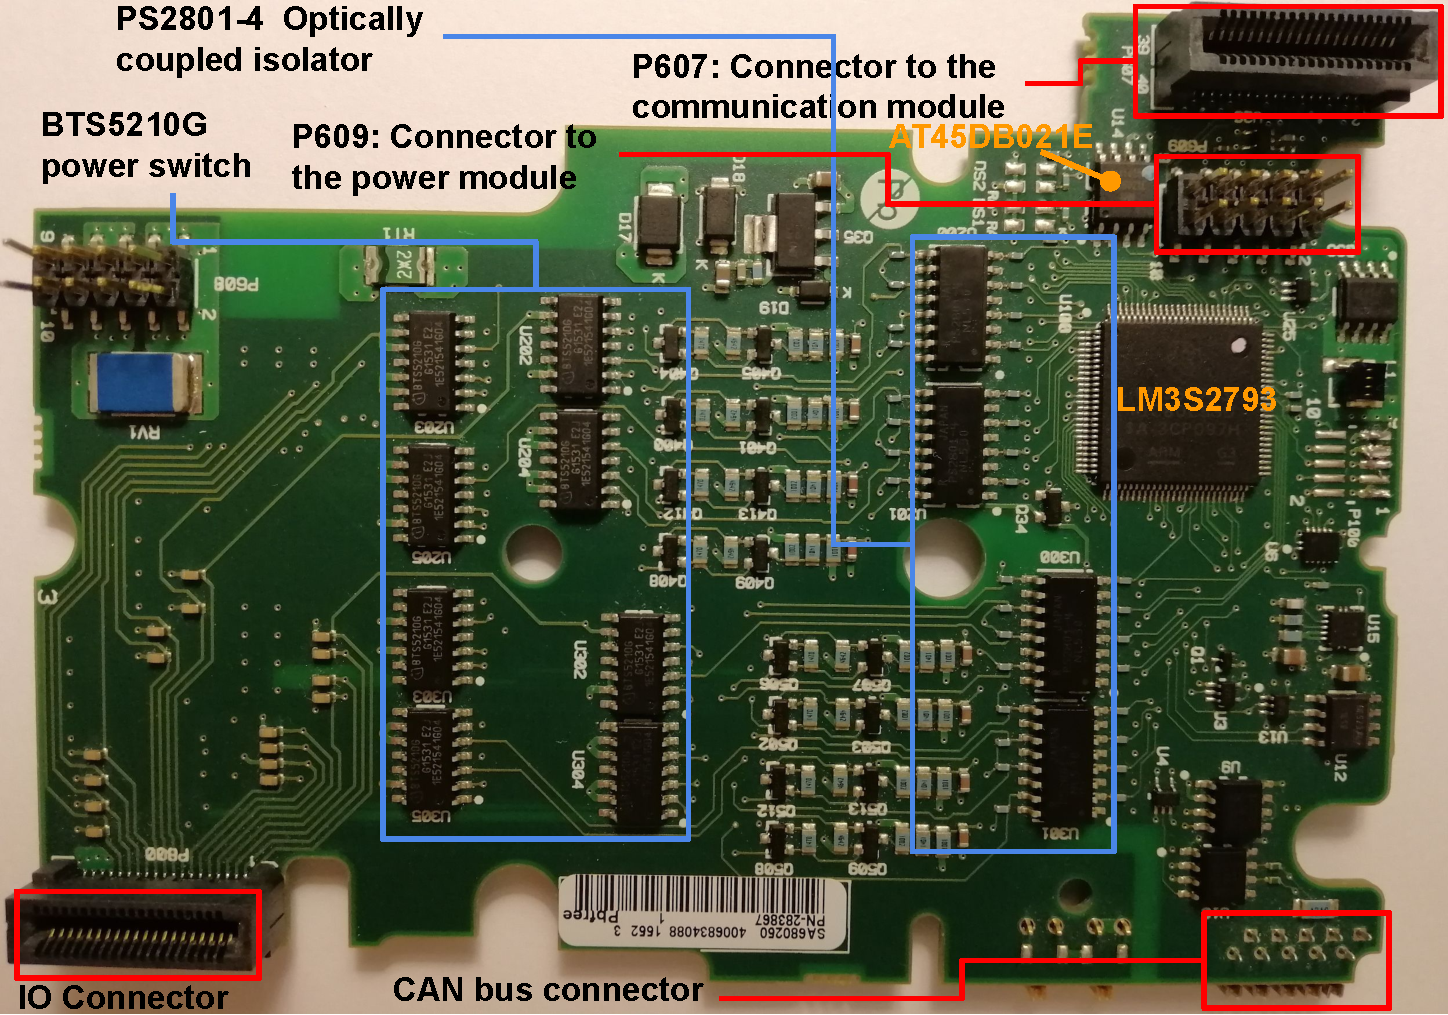
\includegraphics[width=0.47\textwidth]{figures/board3}
	\centering
	\caption{The real-time module reads the input signals, runs the ladder logic, and then drives the output signal according to the result. Therefore this module needs to be connected to all other modules. In addition to the microcontroller and the flash memory, there are power regulators and IO chips on this module. The optically coupled isolators prevent high voltages from affecting the microcontroller when receiving the signal, and the power switches provide the electrical connection between the output pin and the voltage source.}
	\label{fig:board}
\end{figure}


\begin{figure}[th]
	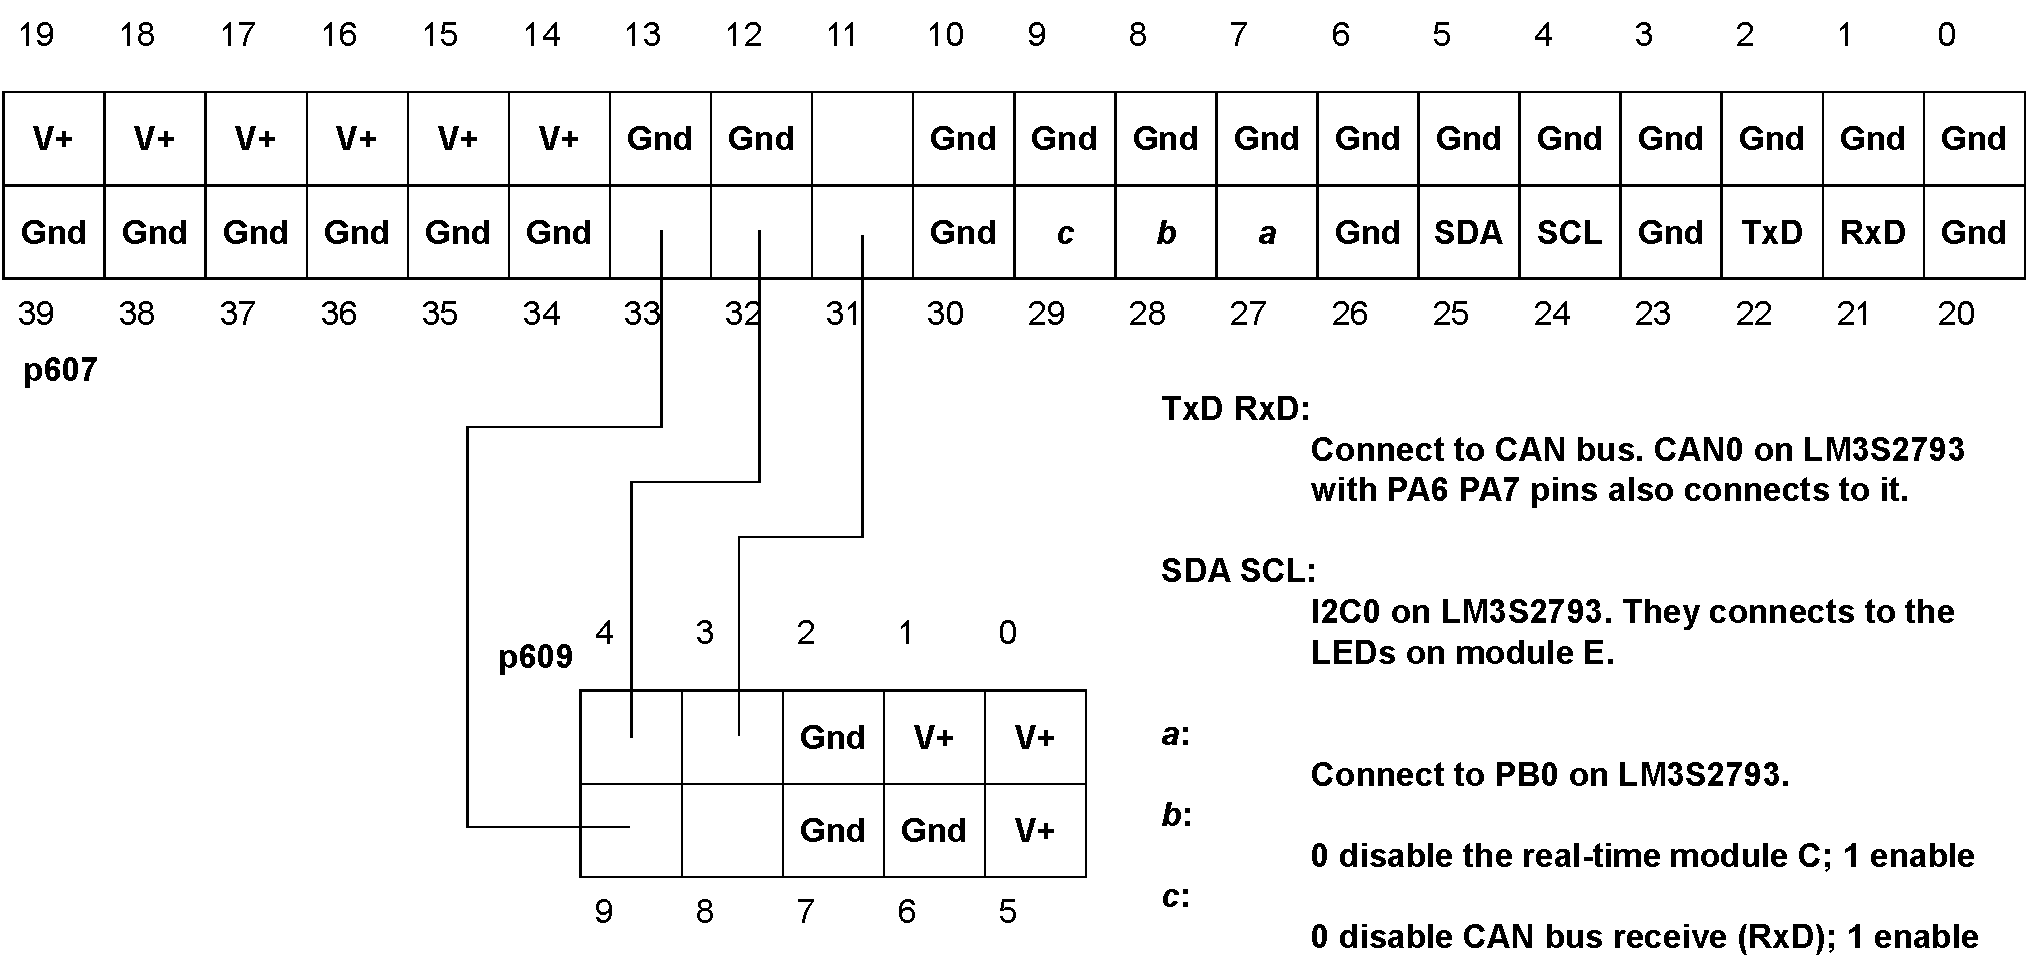
\includegraphics[width=0.47\textwidth]{figures/p607-2}
	\centering
	\caption{The connector between the communication board (module \textbf{B}) and real-time board (module \textbf{C}).  There are many pins, but the majority of them are power and ground. The microcontroller controls the LED module through the P607 connector.  The communication module can block the operation of the entire real-time module through pin28. However, there are still a few pins that we have not figured out their functions. We consider it as one of our further works.}
	\label{fig:p607}
\end{figure}

%As mentioned earlier, on module C, there is a AT45DB21E flash chip. It connects to the microcontroller through SSI0. And it contains one copy of code that will be loaded in once the microcontroller is caught in an unrecoverable error. But by analyzing this interface, we found that the communication module B is not connected to this AT45DB21E flash chip. So we think the code in it is just the backup code used to recover from the fatal error state, and the updated compiled ladder logic is updated by other means.  
%
%By reverse engineering the circuit board and firmware, we identified pin 24 and pin 25 of the connector as the SCL and SDA pin of I2C bus, as shown in~\autoref{fig:p607}. The microcontroller LM3S2793's PAxx PAxx connects LED module E through the communication module B, as shown in~\autoref{fig:modules}.
%
%We also identified that pin 21 and pin 22 are used as CAN bus input and output that come from the communication module B. And pin 29 is used to disable the CAN bus receive signal (RxD). On the CompactLogix PLC 1766, there is only one set of CAN bus for connecting modules. It located on the side of the PLC, it's part of the real-time module, as shown in~\autoref{fig:board}.
%
%
%Both the communication module B and real-time module C are connected to this bus.


\subsection{Design}

Typically, the PLC has a dedicated real-time microcontroller
that handles IO, in this case, module \textbf{D}. It runs minimal code, mainly the compiled ladder logic.  To receive ladder logic update, the communication module \textbf{C} talks to the HMI and then update the real-time microcontroller through the CAN bus. Therefore, to remotely control the PLC's IO, the attacker needs to control further the communication module \textbf{C}, which itself is an independent system usually with a more powerful processor. Moreover, an abnormal traffic filtering mechanism~\cite{kim2016abnormal} also may be deployed to protect ICS networks. Even though we successfully controllers all the embedded system in the PLC and penetrates the network traffic monitors, we still have to face the challenge that a critical infrastructure may run on an isolated local network. Therefore, we choose to use a separate network using GSM.

\begin{figure}[th]
	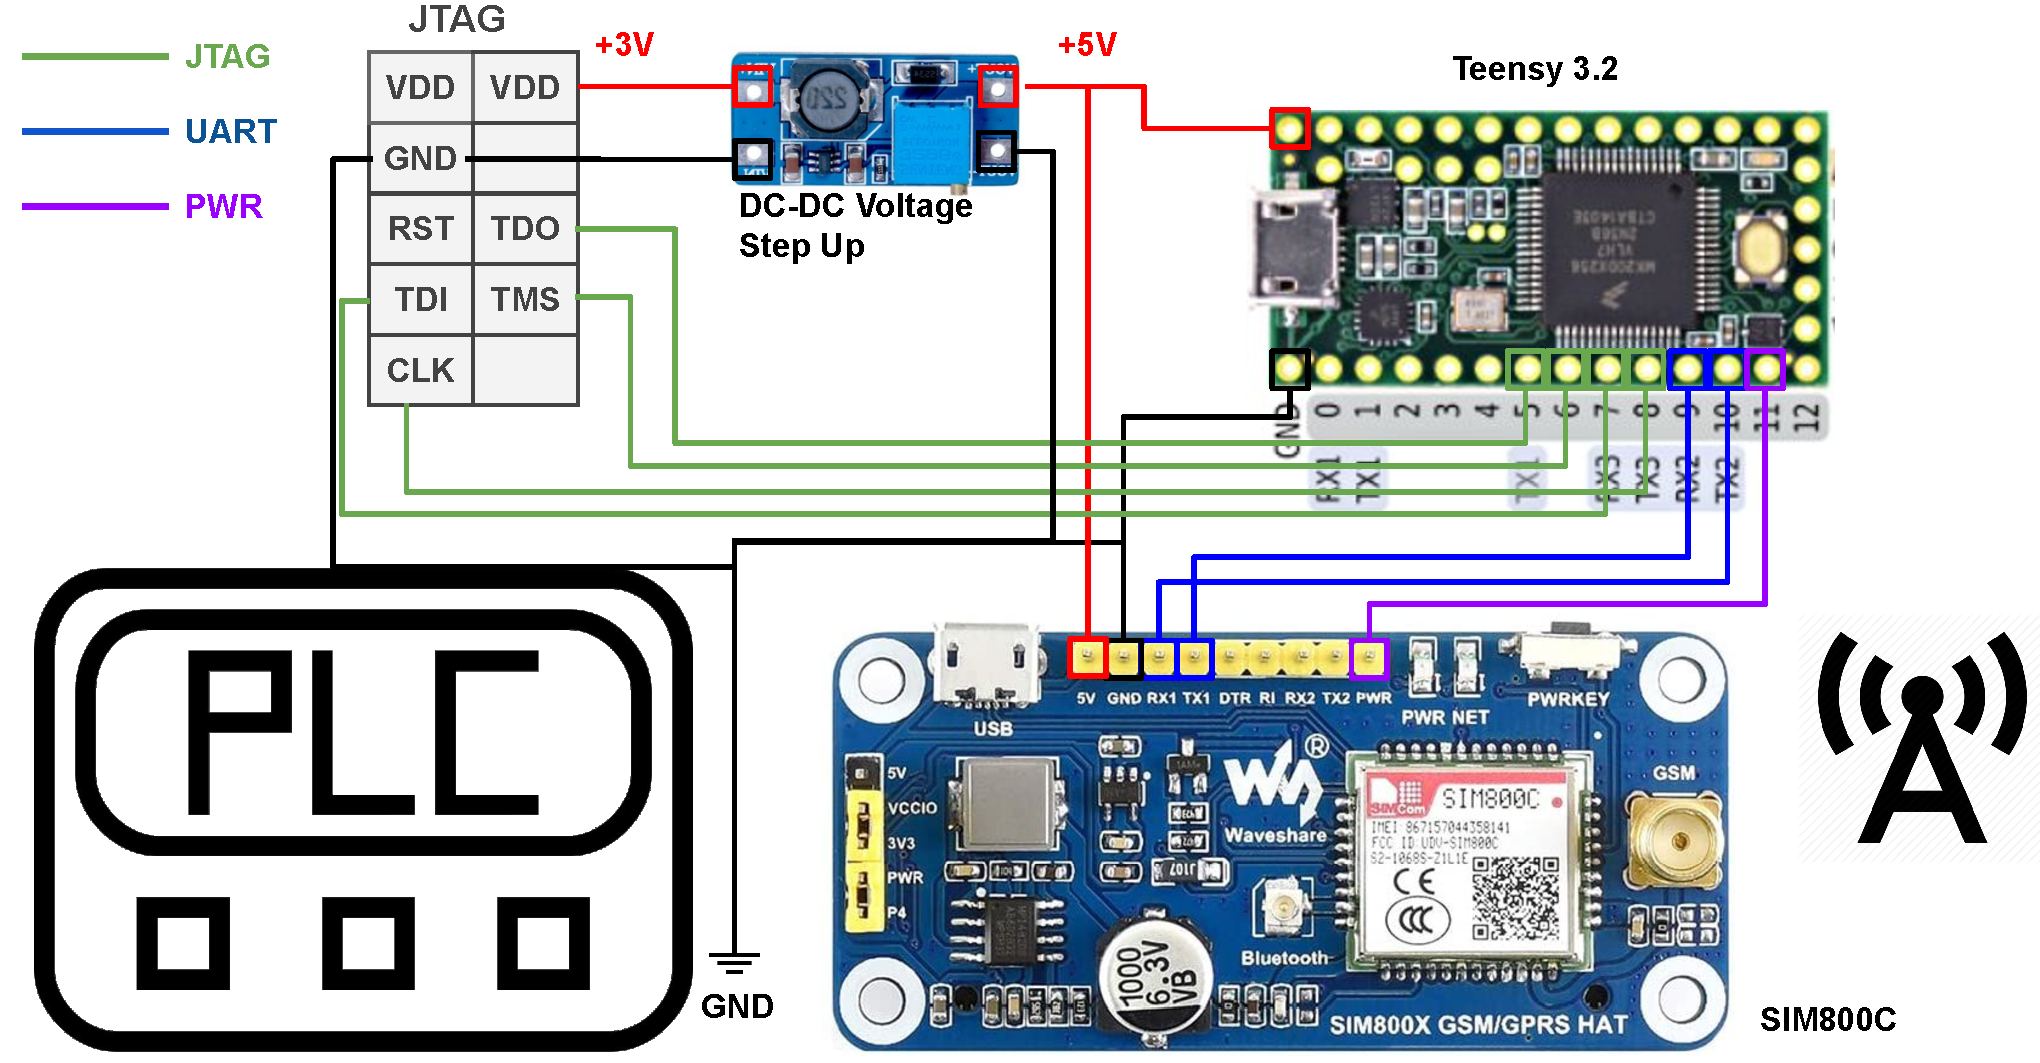
\includegraphics[width=0.47\textwidth]{figures/sim800teensy}
	\centering
	\caption{The power can be drawn from the JTAG pad or directly from the border connector p607. Since the JTAG pad provides the 3 volts source, we also need a DC-DC voltage step-up module that boosts from 3 volts to 5 volts. One GPIO pin from Teensy connects the PWR pin of the SIM800C board. It is used to deliver the power and reset sequence. After SIM800C initialized, the Teensy module sends AT commands through the serial port.}
	\label{fig:sim800teensy}
\end{figure}

The SIM800C is a Quad-Band GSM/GPRS module. It has strong extension capability with interfaces including UART, USB2.0, and GPIO. ~\autoref{fig:sim800teensy} shows that the SIM800C module connects with the Teensy board through a serial port. First, the Teensy boart initializes the cellular module using AT command, connecting to the network. Once a text message is received, the Teensy board reads it and looks for control commands. In such a case,  the command will be parsed as IO operations that eventually turn into particular memory read/write on PLC's GPIO port.
